\section{Models}


\begin{frame}{Benchmark models}

The HAR model is constructed by using the heterogeneity theory of market participants.
\begin{equation}
    \label{eq:har}
    RV_{t+1} = c + \beta^{(d)} RV^{(d)}_{t} + \beta^{(w)} RV^{(w)}_{t} + \beta^{(m)} RV^{(m)}_{t} + X_t' \beta_z + \omega_{t+1}
\end{equation}


Given a return modeled by the following form $r_t = \mu_t + \varepsilon_t$, the GARCH 
process is defined as follow:

\begin{equation}
  \begin{aligned}
  &\varepsilon_t = \sqrt{RV_t} z_t, \quad \varepsilon_t \sim t_\nu(0,1)\\
  &RV_{t+1} = \omega + \alpha \varepsilon_{t}^2 + \beta RV_{t} +  X_{t}' \gamma + \omega_{t+1}
  \end{aligned}
\end{equation}


XGBOOST is an ensemble learning model based on the boosting techniques, where 
a sequence of weak learners, are trained to correct the residual errors of the previous ensemble.\\
$\hspace{47mm} RV_{t+1} = \sum_{k=1}^{K} \eta f_k(x_i)$

    
\end{frame}



\begin{frame}{Interpretable Multivariable LSTM}

The update process of gates, memory cell and hidden states is described using the element-wise multiplication operator $\odot$.
We do not have a single hidden state vectors for each time stamp but multiple hidden states, one for each variable. 
\begin{equation}
  \label{eq:imv_lstm}
  \begin{aligned}
& {\left[\begin{array}{c}
\tilde{\mathbf{i}}_t \\
\tilde{\mathbf{f}}_t \\
\tilde{\mathbf{o}}_t
\end{array}\right]=\sigma\left(\mathcal{W} \circledast \tilde{\mathbf{h}}_{t-1}+\mathcal{U} \circledast \mathbf{x}_t+\mathbf{b}\right)} \\
& \tilde{\mathbf{c}}_t=\tilde{\mathbf{f}}_t \odot \tilde{\mathbf{c}}_{t-1}+\tilde{\mathbf{i}}_t \odot \tilde{\mathbf{j}}_t \\
& \tilde{\mathbf{h}}_t=\tilde{\mathbf{o}}_t \odot \tanh \left(\tilde{\mathbf{c}}_t\right)
\end{aligned}
\end{equation}


    \begin{figure} [H]
    \centering
    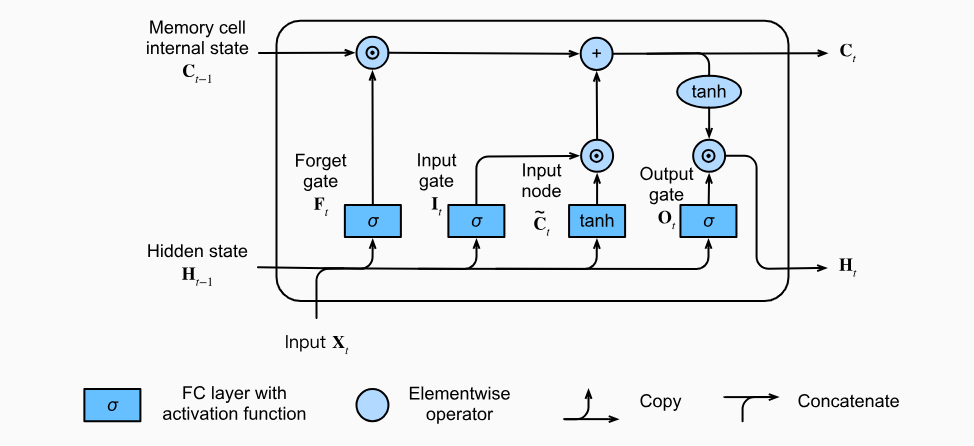
\includegraphics[scale=0.4]{images/LSTM.png}
\end{figure}
    
\end{frame}



\begin{frame}{Interpretable Multivariable LSTM}

The mixture of attention mechanism is composed by:
\begin{itemize}
  \item Temporal-wise attention:
  \begin{equation*}
  \begin{aligned}
    &\alpha^n_t = \frac{\exp\big(f_n(\mathbf{h}^n_t)\big)}{\sum_{k=1}^T \exp\big(f_n(\mathbf{h}^n_k)\big)}\\
    \text{Where } & f_n = tanh(h^n_t W_{\alpha,n} + b_{\alpha,n})
  \end{aligned}
\end{equation*}

  \item Variable-wise attention:
    \begin{equation*}
  \begin{aligned}
    &\beta^n = \frac{\exp\big(f_n(\mathbf{u}^n)\big)}{\sum_{m=1}^N \exp\big(f_m(\mathbf{u}^m)\big)}\\
    \text{where } &f_n = tanh(u^n W_{\beta,n} + b_{\beta,n})
  \end{aligned}
\end{equation*}  
\end{itemize}
Where $\mathbf{g}^n = \sum_{t=1}^T \alpha^n_t \mathbf{h}^n_t$ is the context vector,
$\mathbf{u}^n = \mathbf{h}^n_T \oplus \mathbf{g}^n$ define influence of each variable $n$ to the prediction, and 
$[\mu_n, \sigma_n]=\varphi_n(\mathbf{h}_T^n \oplus \mathbf{g}^n)$ a linear network
 
\vspace{3mm}

The final forecast can be modeled as $p(y_{T+1} \mid X_T) = \sum_{n=1}^N \beta^n \mu_n$\\


\end{frame}


\begin{frame}{Stacking IMV\_LSTM-HAR model}
  
\begin{figure} [H]
    \centering
    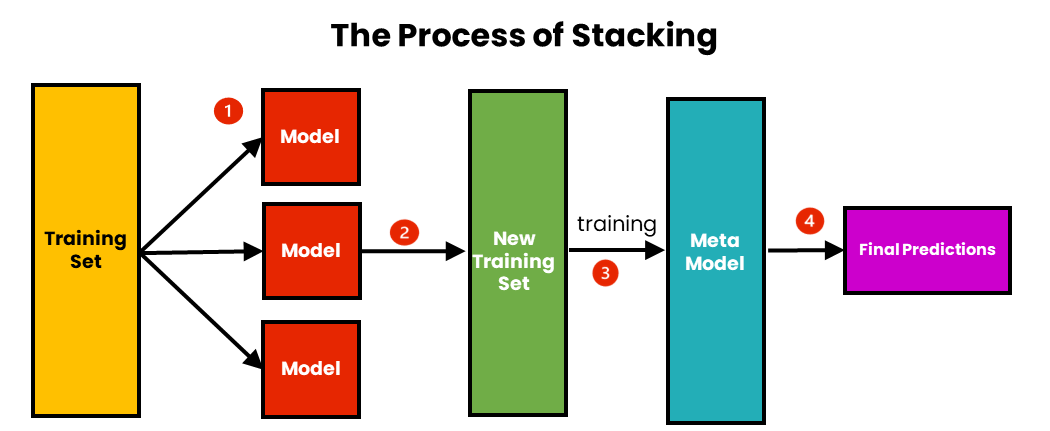
\includegraphics[scale=0.3]{images/stacking.jpg}
\end{figure}


\begin{itemize}
  \item fit HARX and IMV\_LSTM using training set
  \item Produce validation predictions for each model
  \item combine prediction data into a new dataset whose features are the predictions of each horizon from each model
  \item fit the meta learner linear regression model to combine predictions
\end{itemize}


\end{frame}


